% igs2ejournalguide.tex
% v4.00 3-sept-2015

\NeedsTeXFormat{LaTeX2e}

% check that the math fits the two-column format:
 \documentclass[twocolumn,letterpaper]{igs}

% but use this version when submitting your article:
 %\documentclass[review,oneside]{igs}


  \usepackage{igsnatbib}
\usepackage{lmodern}
\usepackage{amsmath,amssymb,amsthm}
\usepackage{wrapfig}
\usepackage{enumitem}
\usepackage{multirow}
\usepackage{tabularx}
\usepackage{booktabs}
\usepackage{lscape}
\usepackage{color}
\usepackage{graphicx}
\usepackage{subcaption}


\definecolor{CL}{rgb}{ 0,    0.4470,    0.7410}
\definecolor{CT}{rgb}{0.8500,    0.3250,    0.0980}
\definecolor{CR}{rgb}{0.9290,    0.6940,    0.1250}
\definecolor{HG}{rgb}{ 0.4940,    0.1840,    0.5560}
\definecolor{HC}{rgb}{0.4660 ,   0.6740 ,   0.1880}
\definecolor{RN}{rgb}{0.3010 ,   0.7450 ,   0.9330}

 


\begin{document}

\title[Optimal snow-survey design for estimating winter balance]{Optimal snow-survey design for the estimation of winter balance on alpine glaciers}

\author[Pulwicki and Flowers]{Alexandra PULWICKI,$^a$
  Gwenn E. FLOWERS,$^b$}

\affiliation{%
$^a$ Department of Earth Sciences, Simon Fraser University, 8888 University Drive, Burnaby, BC, V5A 1S6, Canada\\
  $<$apulwick@sfu.ca$>$\\
 $^b$ Department of Earth Sciences, Simon Fraser University, 8888 University Drive, Burnaby, BC, V5A 1S6, Canada\\
  $<$gflowers@sfu.ca$>$ }

%%%%%%%%%%%%%%%%%%%%%%%%%%%%%%%%%
%	ABSTRACT
%%%%%%%%%%%%%%%%%%%%%%%%%%%%%%%%%

\abstract{Efficient collection of snow depth and density data is central to a successful snow survey and to accurately estimating  the winter surface mass balance of glaciers. Simultaneously extensive, high resolution and accurate snow-depth measurements are almost impossible to obtain on glaciers, so surveys should be designed to optimize measurement configuration and spacing. 
Using data from three small glaciers in the St. Elias Mountains of Yukon, Canada,
we consider numerous survey designs, comprising six possible spatial patterns of snow-depth sampling and 8--200+  sampling locations per glacier. We then use linear regression on topographic parameters to generate glacier-wide distributions of winter balance. In tests using both real and synthetic data, we find that the common centreline survey design produces the poorest results by all metrics for all three glaciers. Adding lateral transects to the centreline survey, or using the ``hourglass'' sampling pattern, yields greatly improved accuracy while retaining efficiency. Random sampling also performs well but compromises efficiency.  
In many cases, error decreases sharply with sample size up to $\sim$10 and more slowly thereafter, with little further reduction for sample sizes $\gtrsim 30$. 

\vspace{0.3cm} Keywords: {\normalfont glacier; alpine; snow survey; optimal design; glacier mass balance; St. Elias Mountains}}

\maketitle

%%%%%%%%%%%%%%%%%%%%%%%%%%%%%%%%%
%	INTRODUCTION
%%%%%%%%%%%%%%%%%%%%%%%%%%%%%%%%%
\section{Introduction}

\begin{figure*}
	\centering
	\includegraphics[width =\textwidth]{Pulwicki_Fig1.pdf}\\
	\caption{Study area location and sampling patterns for Glaciers 4, 2 and 13. (Left) Study region in the Donjek Range of the St. Elias Mountains, Yukon, Canada (inset). Imagery from Sentinel-2A (29 August 2013, Copernicus Sentinel data 2013). (Right) Spatial sampling patterns:  centreline and transverse profiles (blue dots), hourglass with inscribed circle (orange dots). Also shown are locations of snow-density measurements  (green squares), ice-flow directions (arrows), approximate location of ELA on each glacier (black dashed lines) and elevation contours (grey) with contour interval of 50\,m.}
	\label{fig:Sampling}
\end{figure*} 

Estimates of basin-wide seasonal snow accumulation are critical for monitoring glacier mass balance and for predicting the availability and timing of surface runoff, especially in mountainous regions. The net accumulation of snow on a glacier over a winter season is known as the winter surface mass balance, or ``winter balance'' and is typically reported in meters of water equivalent (m\,w.e.) \citep{Cogley2011}. Winter balance accounts for half of the seasonally resolved mass balance, initializes ablation conditions and affects energy and mass exchange between the land and atmosphere \citep[e.g.][]{Hock2005, Reveillet2016}. 

Optimal survey designs for snow depth are central to accurately estimating snow distribution and mass balance from \textit{in situ} measurements. Measuring snow depth and travelling between measurement locations is both time consuming and can disturb the snow, so care must be taken to choose a survey design that avoids bias, allows for the greatest variability to be measured and minimizes distance travelled \citep[e.g.][]{Shea2010,Kinar2015}. Moreover, the period of seasonal maximum snow depth can be brief, further motivating the need for time-efficient survey designs. 

There are a number of different spatial sampling patterns that have been employed to obtain point measurements of snow depth, including pure random \citep[e.g.][]{Elder1991}, linear random \cite[e.g.][]{Shea2010}, nested \citep[e.g.][]{Schweizer2008}, gridded random \citep[e.g.][]{Bellaire2008, Elder2009, Bellaire2011} and gridded \citep[e.g.][]{Molotch2005a, Kronholm2007, Lopez2011}. Sampling schemes that incorporate randomness are favourable because they limit sampling bias by varying sample spacing and direction. However, they are less efficient than designs that incorporate grids. Grid-based designs minimize travel distance but measurements are biased by regularly spaced intervals and linear orientations which can result in an under-representation of  snow-depth variability \citep{Kronholm2007}.

Snow surveys on glaciers are conducted to estimate winter balance, with multi-year sampling programs established to monitor temporal changes in winter balance. An optimal survey design requires (1) a sampling scheme that captures spatial variability and minimizes travel distance and (2) identification of the minimum number of measurement locations needed to estimate winter balance to the desired precision.  Optimization of winter-balance survey design is rarely investigated because the locations of snow-depth measurements are often dictated by field resources and logistics. 
Few studies have investigated the number of measurement locations needed to effectively sample mass-balance distributions \citep[c.f.][]{Fountain1999,Walmsley2015,Surjanovic2016}. The sampling patterns used for most winter-balance programs do not include randomness, and measurements are typically made along the glacier centreline \citep[e.g.][]{Kaser2003} to capture expected orographic effects \citep[e.g.][]{Grunewald2014}. However, centreline surveys are known to underestimate winter balance, so transverse profiles are often added to improve the reliability of the sampling scheme \citep[e.g.][]{Walmsley2015}. An hourglass with an inscribed circle (personal communication from C. Parr, 2016) is an alternative sampling scheme that captures changes in winter balance with elevation while avoiding the centreline bias, and is easy to travel. To our knowledge, no study has yet compared the performance of these different sampling schemes in estimating winter balance.

The goal of this work is to determine the optimal survey design for estimating glacier-wide winter balance. We consider both the spatial sampling scheme and the number of measurement locations in defining the optimal design. For three alpine glaciers in the St. Elias Mountains of Yukon, Canada, we explore the effects of survey design on the accuracy of estimated glacier-wide winter balance in tests with synthetic and real data.

%%%%%%%%%%%%%%%%%%%%%%%%%%%%%%%%%
%	STUDY SITE
%%%%%%%%%%%%%%%%%%%%%%%%%%%%%%%%%

\section{Study site}

We investigate winter-balance survey design for three unnamed glaciers in the Donjek Range of southwest Yukon, Canada. Situated on the northern flanks of the St. Elias Mountains, which rise sharply from the Pacific Ocean, the Donjek Range experiences a continental climate. Monitoring snow distribution and glacier mass balance in the St. Elias Mountains began in the 1950s and 1960s with a series of research programs, including Project ``Snow Cornice''  and the Icefield Ranges Research Project \citep{Wood1948, Danby2003}. More recent studies have focused on studies of individual alpine glaciers \citep[e.g.][]{Clarke2014,Flowers2014} as well as regional glacier mass balance and dynamics \citep[e.g.][]{Arendt2008, Burgess2013,Waechter2015}. 

Glacier 4, Glacier 2 and Glacier 13 (labelling adopted from \cite{Crompton2016}) are small alpine glaciers (3.8--12.6\,km$^2$) with simple geometries. The elevation of these glaciers ranges from 1900 to 3100\,m\,a.s.l. and ELAs are located at $\sim$2500\,m. The glaciers are generally oriented southeast-northwest in steep-walled valleys. We suspect that all three glaciers are polythermal, based on a targeted study of Glacier 2 \citep{Wilson2013} and related theoretical modelling \citep{Wilson2013a}. A detailed analysis of winter-balance estimation on these glaciers is presented by \cite{Pulwicki2017}.


%%%%%%%%%%%%%%%%%%%%%%%%%%%%%%%%%
%	METHODS
%%%%%%%%%%%%%%%%%%%%%%%%%%%%%%%%%
\begin{figure*}
	\centering
	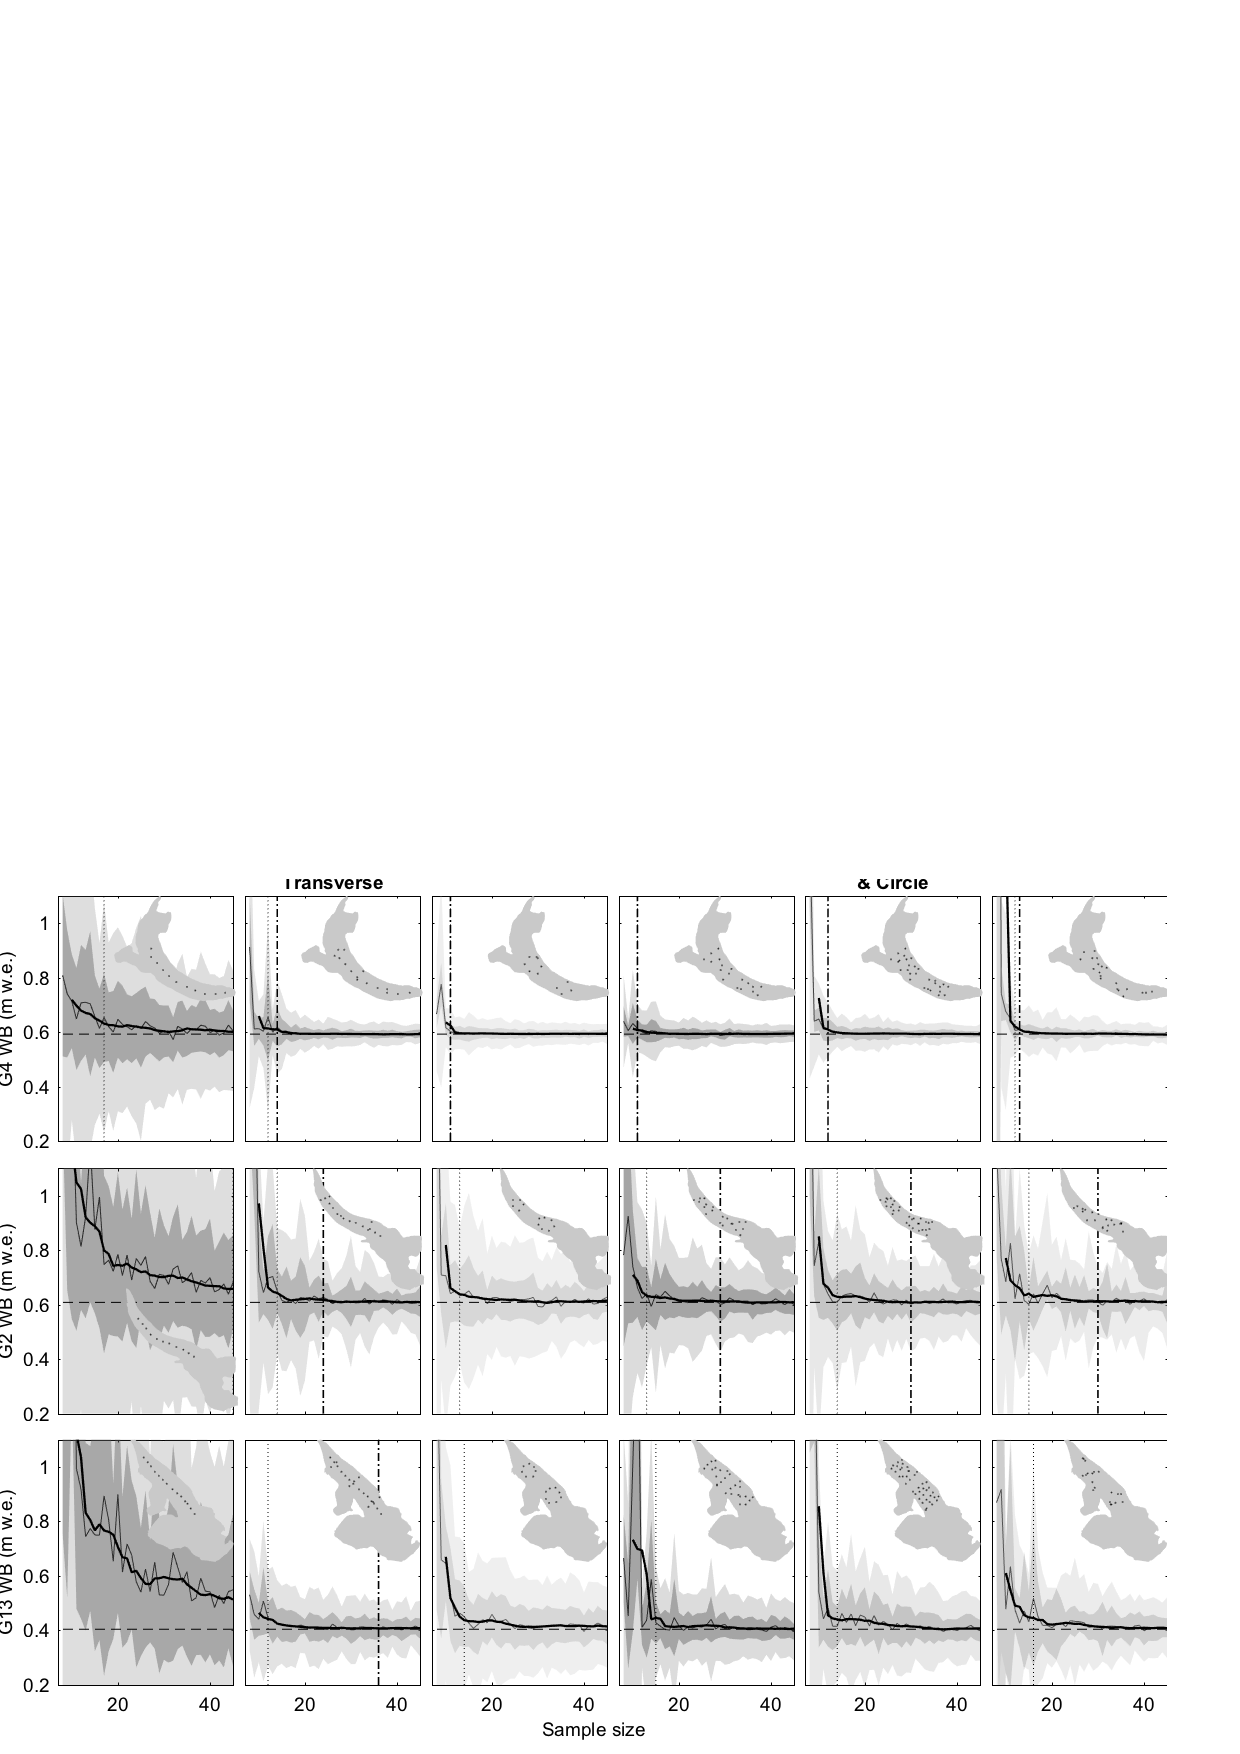
\includegraphics[width =0.9\textwidth]{Pulwicki_Fig2.pdf}\\
	\caption{Synthetic sampling patterns on the three study glaciers. All synthetic sampling locations (small black dots) and a subset of synthetic sampling locations ($n=15$, open circles) are shown for each sampling pattern. The random pattern shows a total of 200 synthetic sampling locations. Sampling patterns are overlain on the synthetic distribution of winter balance (WB) in colour. } 
       \label{fig:SyntheticSampleDesign}
\end{figure*}

\section{Methods}

Below we outline the process of determining point-scale and grid-scale values of winter balance from snow depth and density measurements. We then describe the production of gridded synthetic distributions of winter balance for each of the three study glaciers, from which synthetic sample datasets are extracted. Finally, we present our strategy for evaluating survey design with real and synthetic data, using specific performance metrics. 

\subsection{Field measurements}

Point-scale values of winter balance are obtained from direct measurements of snow depth and density (Figure \ref{fig:Sampling}). Snow depth was measured using  3.2\,m graduated aluminium avalanche probes. Measurement locations followed linear and curvilinear transects in various spatial patterns termed ``centreline'' and ``transverse'' transects, ``hourglass'' and ``circle''. 
Centreline transects, alone or combined with transverse transects, comprise the most common survey designs used in winter-balance studies \citep[e.g.][]{Kaser2002, Machguth2006}. The centreline transect aims to capture changes in winter balance with elevation, while transverse transects provide some characterization of lateral variations in winter balance. The hourglass with inscribed circle allows for sampling in multiple directions and easy travel (personal communication from C. Parr, 2016). 

Sampling patterns were similar between study glaciers, with a sample spacing of 10--60\,m dictated by protocols for safe glacier travel. Each observer made 3--4 individual depth measurements within $\sim$1\,m at each survey location; these measurements were averaged to obtain a single value. Snow-depth measurements were largely restricted to the ablation area, where the clear distinction between snow and ice ensures that only snow from the most recent accumulation season is measured. In total, we collected more than 9000 snow-depth measurements throughout the study area. 

Snowpit-density profiles were measured using a wedge cutter and spring scale at three locations on each glacier that were distributed in elevation. A mean density was then calculated for each glacier and used to convert snow depth at all measurement locations to values of point-scale winter balance. The mean density and standard deviation were 348$\pm$13\,kg\,m$^{-3}$ on Glacier 4, 333$\pm$26\,kg\,m$^{-3}$ on Glacier 2 and 349$\pm$38\,kg\,m$^{-3}$ on Glacier 13. All point-scale values of winter balance located within a common digital elevation model (DEM) gridcell ($40\times40$\,m) were averaged to obtain a single value of winter balance in each sampled gridcell. A detailed analysis of uncertainty in winter balance due to the treatment of snow density can be found in \cite{Pulwicki2017}.

\subsection{Tests with synthetic data}

A synthetic glacier-wide distribution of winter balance is obtained for each study glacier by linear regression of the gridcell-averaged values of winter balance (obtained as described above) on topographic parameters derived from a SPIRIT SPOT-5 DEM \citep{Korona2009}. These parameters include commonly used quantities such as elevation, slope, aspect, distance from glacier centreline, ``northness'', curvature and a wind redistribution parameter \citep[e.g.][]{McGrath2015}. The regression is used, along with cross-validation and Bayesian model averaging, to obtain a set of regression coefficients for each glacier \citep{Pulwicki2017}. The resulting distribution of winter balance, hereafter referred to as the ``synthetic distribution of winter balance'' is determined by multiplying fitted regression coefficients by the corresponding topographic parameters for each gridcell in the DEM. We use the regression as an emulator to generate realistic winter-balance distributions that we can treat as synthetic data. 

Synthetic data are used to evaluate survey design, including the spatial sampling pattern and the number of measurement locations or sample size. 
We investigate various survey designs that are unique combinations of six different sampling patterns: centreline, centreline and transverse transects, circle, hourglass, hourglass with inscribed circle and random. The random pattern is restricted to the area encompassed by the original field measurements (Figure \ref{fig:Sampling}). 
All sampling patterns are restricted to the ablation area, where terrain is accessible and measurements of snow depth are generally unambiguous. 
For each sampling pattern we investigate the effect of sample size $n$, where $n$ ranges from a minimum of eight (constrained by the use of seven topographic parameters in the interpolation) to a maximum determined by the number of gridcells sampled by a given pattern (ranging from 57 to 228). 

To generate a synthetic sample size ($n$) for a given sampling pattern (e.g. hourglass), we extract $n$ regularly spaced values from the chosen sampling pattern within the glacier-wide synthetic distribution of winter balance. 
The geographic locations of the patterns are fixed based on the original field measurements.    
We then add low or high noise to the synthetic sample set. Low noise is defined by a normal distribution with zero mean and a standard deviation derived from a series of high-density subgrid-scale measurements of winter balance on each glacier \citep{Pulwicki2017}.  
High noise is similarly defined, but with the standard deviation three times that of low noise. This value is approximately equal to that derived by \citet{Pulwicki2017} to represent multiple sources of uncertainty including subgrid-scale variability (as in the low-noise case), the assignment of snow density in the conversion of snow depth to winter balance and measurement interpolation.
For each synthetic sample of winter balance, a randomly chosen value from the high- or low-noise distribution is added to the sample value. Any negative values of synthetic data are set to zero. 

To assess the performance of a given survey design (sampling pattern and sample size), we compare the original synthetic distribution of winter balance to that obtained when the topographic regression is performed using only the noisy synthetic sample set. 
Since the noise is sampled randomly from a distribution, we repeat the regression to create 100 realizations of ``estimated winter balance'' from which we can calculate a mean and standard deviation. Comparison of the ``synthetic'' and ``estimated'' winter balances allows us to assess the accuracy of the estimated value, and its sensitivity to noise, for a given survey design. 
The utility of the results is limited by the extent to which the simulated distribution represents a plausible reality.   
 
 \subsection{Tests with real data}
 
 Using real data offers an alternative way to evaluate survey design, and provides a check on the results obtained in the synthetic tests. 
Here we aim to test how well the estimated winter balance compares with field measurements, as well as how it compares to winter balance estimated using all available data, as a function of sampling pattern and sample size. 
In this series of tests, we extract subsets of $n$ regularly spaced samples of the observed winter balance (as described in ``Field measurements'') from individual sampling patterns (e.g. hourglass with inscribed circle) and use each subset of observed values to generate an ``estimated winter balance'' with a linear regression as described above. Because these values are real data, they already contain noise. 
We then repeat the regression 100 times with randomly selected subsets of $n$ values, which are not regularly spaced. From these 100 realizations we calculate a mean and standard deviation of the estimated winter balance. We then compute the RMSE between all observed values of winter balance and the co-located estimates of winter balance. This comparison allows us to assess the accuracy of predicted values of winter balance, at the locations of the original field measurements, for a given survey design with regularly and randomly spaced data. 


 \subsection{Performance metrics}
 
To quantify the performance of each survey design, we use two metrics. The first metric we term ``convergence'', defined as the sample size ($n_{\rm c}$) needed to obtain a mean estimated glacier-wide winter balance within 5\% of the target value in the synthetic tests, or RMSE within 5\% of the target value in the comparison with real data. In the latter case, the target value is the RMSE achieved when all available data are used to estimate winter balance.
To determine $n_{\rm c}$ we smooth the mean estimated values of glacier-wide winter balance or RMSE as a function of $n$ to avoid spurious results arising from the random noise added to the synthetic samples or the random sample selection of the observed values.
Convergence is a metric that describes the minimum number of measurement locations required to produce an accurate estimate of winter balance (within 5\%) in the synthetic tests, and a precise estimate of winter balance (within 5\%) in the tests with real data. 

The second metric we term ``variability'', defined as the sample size ($n_{\rm v}$) needed to obtain a standard deviation of the estimated glacier-wide winter balance within 25\% of the target value in the synthetic tests with high noise, or standard deviation of RMSE within 25\% of the target value in the comparison with real data. We again smooth the standard deviation of estimated values of glacier-wide winter balance or RMSE as a function of $n$, in order to determine $n_{\rm v}$. 
``Variability'' is a metric that describes the sensitivity of the estimated winter balance to noise in the synthetic tests and sampling locations in the comparisons with real data.
We also compute the total travel distance required to obtain the measurements required for a given survey design. An efficient survey will have low values of  $n_{\rm c}$ and $n_{\rm v}$ as well as a short travel distance. 

%%%%%%%%%%%%%%%%%%%%%%%%%%%%%%%%%%%%%%%%%%%
%%  RESULTS
%%%%%%%%%%%%%%%%%%%%%%%%%%%%%%%%%%%%%%%%%%%
\section{Results }

Below we describe the performance of the different survey designs (sampling patterns and sample sizes) for each glacier, and rank each sampling pattern based on the performance criteria $n_{\rm c}$ and $n_{\rm v}$, in the synthetic- and real-data tests. 

\subsection{Tests with synthetic data}

\begin{figure*}
	\centering
	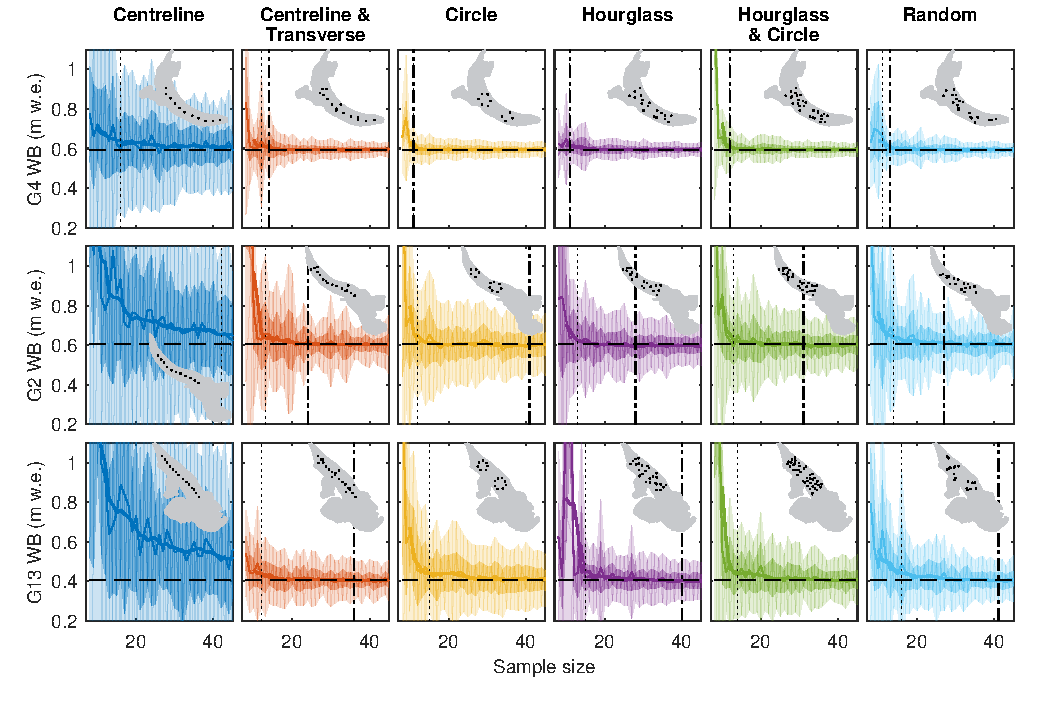
\includegraphics[width =\textwidth]{Pulwicki_Fig3.pdf}\\
	\caption{Glacier-wide winter balance (WB) estimated with various sampling patterns (columns) and sample sizes (x-axes) for Glacier 4 (top row), Glacier 2 (middle row) and Glacier 13 (bottom row). Insets show example sampling patterns. Bold solid lines are smoothed mean values of WB  (fine solid lines) estimated from 100 linear regressions of synthetic samples of WB on topographic parameters for each sampling pattern and sample sizes from 8 to $> 45$ (x-axes). Dark and light shading indicate the standard deviation in estimated WB for low- and high-noise cases, respectively. Horizontal dashed lines indicate the synthetic target value of glacier-wide WB. Vertical dotted lines show sample size $n_{\rm c}$ that achieves an accuracy of 5\% (difference between smoothed mean and target value). Vertical dot-dashed lines show sample size $n_{\rm v}$ for which the standard deviation comes within 25\% of the target value for the high-noise case. Not all sampling patterns have $n_{\rm c}$ and $n_{\rm v}$ within the range of samples sizes shown.}
	\label{fig:SyntheticObsWB}
\end{figure*}


Based on the synthetic tests, the most accurate sampling patterns are circle (CR), hourglass (HG) or centreline \& transect (CT), depending on the metric used ($n_{\rm c}$ or $n_{\rm v}$) and the glacier (Figure \ref{fig:SyntheticObsWB}, Table \ref{tab:SynthPatternRanks}). 
With all sampling patterns, winter balance is overestimated at low sample sizes.
For Glacier 4, circle, hourglass and random converge equally quickly ($n_{\rm c}=11$) to the target synthetic value of glacier-wide winter balance, with circle and hourglass exhibiting the least sensitivity to noise ($n_{\rm v}=11$). For Glacier 13, centreline \& transverse is best, with $n_{\rm c}=12$ and $n_{\rm v}=36$. For Glacier 2, circle converges most quickly ($n_{\rm c}=12$) but variability is minimized with centreline \& transverse ($n_{\rm v}=24$). Among these four sampling patterns, circle requires the least travel and centreline \& transverse and random the most (Table \ref{tab:SynthPatternRanks}, bottom three rows). 
If using hourglass, circle, hourglass \& circle or centerline \& transverse sampling patterns, a sample size $\leq 15$ is sufficient for convergence of the mean to the target synthetic value of winter balance for all glaciers. 
To ensure convergence in the presence of high noise for all glaciers, a sample size of  $\leq 36$ is sufficient for centerline \& transverse, $ \leq 40$ for hourglass and $\leq 53$ for hourglass \& circle; for circle this value is 103. 
The values of $n_{\rm v}$ are much lower for Glaciers 4 and 2 than for Glacier 13.   
Of note is the fact that hourglass, circle and hourglass \& circle perform similarly as judged by convergence ($n_{\rm c}$) for all glaciers, and variability ($n_{\rm v}$) for Glacier 4; circle performs much more poorly in terms of variability for Glaciers 2 and 13.

\begin{table*}[]
\centering
\caption{Synthetic data tests. Ranking of survey designs from 1 to 6 (left to right) for Glaciers 4, 2 and 13 (G4, G2, G13) based on metrics (see text) $n_{\rm c}$ (top three rows) and $n_{\rm v}$ (middle three rows) as well as travel distance ($d$) required to perform survey (bottom three rows). Sampling patterns are: centreline (CL), centreline \& transverse (CT), circle (CR), hourglass (HG), hourglass \& circle (HC) and random (RN). Colours follow figures. Values in parentheses are $n_{\rm c}$, $n_{\rm v}$ or travel distance (km). Travel distances given for random sampling scheme are averages.}
\label{tab:SynthPatternRanks}
\begin{tabular}{clclclclclclcl}
\hline
          && \textbf{1} && \textbf{2} && \textbf{3} && \textbf{4} && \textbf{5} && \textbf{6} \\
 \hline
                & \textbf{G4}    & \textcolor{CR}{CR}, \textcolor{HG}{HG}, \textcolor{RN}{RN}         & (11)         &          &         & 	& 	&  \textcolor{CT}{CT}, \textcolor{HC}{HC}         & (12)                 &          &  & \textcolor{CL}{CL} & (16) \\
$n_{\rm c}$         & \textbf{G2}   & \textcolor{CR}{CR}         & (12)                   &  \textcolor{HG}{HG}, \textcolor{HC}{HC},\textcolor{CT}{CT}          & (13)         &      &  & &         & \textcolor{RN}{RN}        & (14)  &   \textcolor{CL}{CL} & (42) \\
                & \textbf{G13} & \textcolor{CT}{CT}         & (12)         & \textcolor{HC}{HC} & (14)         &    \textcolor{HG}{HG}, \textcolor{CR}{CR}               & (15)         & & &  \textcolor{RN}{RN}                &        (16)          & \textcolor{CL}{CL} & (100) \\
\hline
                & \textbf{G4}   & \textcolor{CR}{CR},  \textcolor{HG}{HG}         & (11)         &         &           & \textcolor{HC}{HC}         & (12)         & \textcolor{RN}{RN}                 & (13)         & \textcolor{CT}{CT} & (14) & \textcolor{CL}{CL} & (--) \\
$n_{\rm v}$         & \textbf{G2}   & \textcolor{CT}{CT}         & (24)         &  \textcolor{RN}{RN}         & (27)    &	 \textcolor{HG}{HG}  & (28)    & \textcolor{HC}{HC}        & (31)              &  \textcolor{CR}{CR}         & (41) & \textcolor{CL}{CL} & (--) \\
                & \textbf{G13} & \textcolor{CT}{CT}         & (36)         & \textcolor{HG}{HG}         & (40)         & \textcolor{RN}{RN}                 & (50)         &    \textcolor{HC}{HC}      &     (53)     & \textcolor{CR}{CR}         & (102) & \textcolor{CL}{CL} & (--) \\
\hline
                & \textbf{G4}   & \textcolor{CR}{CR}         & (4.8) & \textcolor{CL}{CL}         & (6.3) & \textcolor{HG}{HG}                 & (6.9)         & \textcolor{RN}{RN}         & ($\sim$7.9) & \textcolor{CT}{CT}         & (8.3) & \textcolor{HC}{HC} & (11.1) \\
$d$        & \textbf{G2}   & \textcolor{CL}{CL}         & (4.3) & \textcolor{CR}{CR}         & (5.7) & \textcolor{HG}{HG}                 & (8.4)         & \textcolor{CT}{CT} & (8.6)         & \textcolor{RN}{RN}                 & ($\sim$9.2) & \textcolor{HC}{HC} & (12.5) \\
                & \textbf{G13} & \textcolor{CR}{CR}         & (7.0) & \textcolor{CL}{CL}         & (8.0) & \textcolor{HG}{HG}                 & (10.6)         & \textcolor{CT}{CT} & (11.0)         & \textcolor{RN}{RN}                 & ($\sim$11.3) & \textcolor{HC}{HC} & (16.8)\\
\hline
\end{tabular}
\end{table*}


\begin{figure*}
	\centering
	\includegraphics[width =\textwidth]{Pulwicki_Fig4.pdf}\\
	\caption{Distributed RMSE between synthetic target distribution of winter balance and the mean winter balance estimated with various sampling patterns (columns), $n=40$ and 100 regressions of the high-noise sample set for Glacier 4 (top row), Glacier 2 (middle row) and Glacier 13 (bottom row). Numbers indicate glacier-wide RMSE. Synthetic sample locations are shown as black dots.}
	\label{fig:SynObsRMSEmap}
\end{figure*}


The remaining sampling patterns, centreline (CL) and random (RN), are less accurate in estimating the synthetic winter balance, though random performs comparably to the others particularly as assessed by convergence $n_{\rm c}$. 
Of all sampling patterns, centreline is decisively the worst, ranked last for all glaciers for both $n_{\rm c}$ and $n_{\rm v}$. Winter balance estimated with a centreline sampling pattern is highly sensitive to noise for all glaciers and only achieves convergence to the target synthetic value for low sample sizes ($n_{\rm c}=17$) on Glacier 4. 

Although the convergence patterns are generally similar between glaciers, the sample sizes needed to accurately estimate winter balance ($n_{\rm c}$) and ensure convergence in the presence of high noise ($n_{\rm v}$) are smallest for Glacier 4 and largest for Glacier 13 for all sampling patterns (compare top row to bottom row in Figure  \ref{fig:SyntheticObsWB}). The RMSE between estimated and synthetic values of winter balance is also greater on Glaciers 2 and 13 than on Glacier 4, especially in the accumulation area (Figure \ref{fig:SynObsRMSEmap}). When the centreline pattern is used, the RMSE is high over a large areal fraction of the glacier (Figure \ref{fig:SynObsRMSEmap}).

\subsection{Tests with real data}

\begin{figure*}
	\centering
	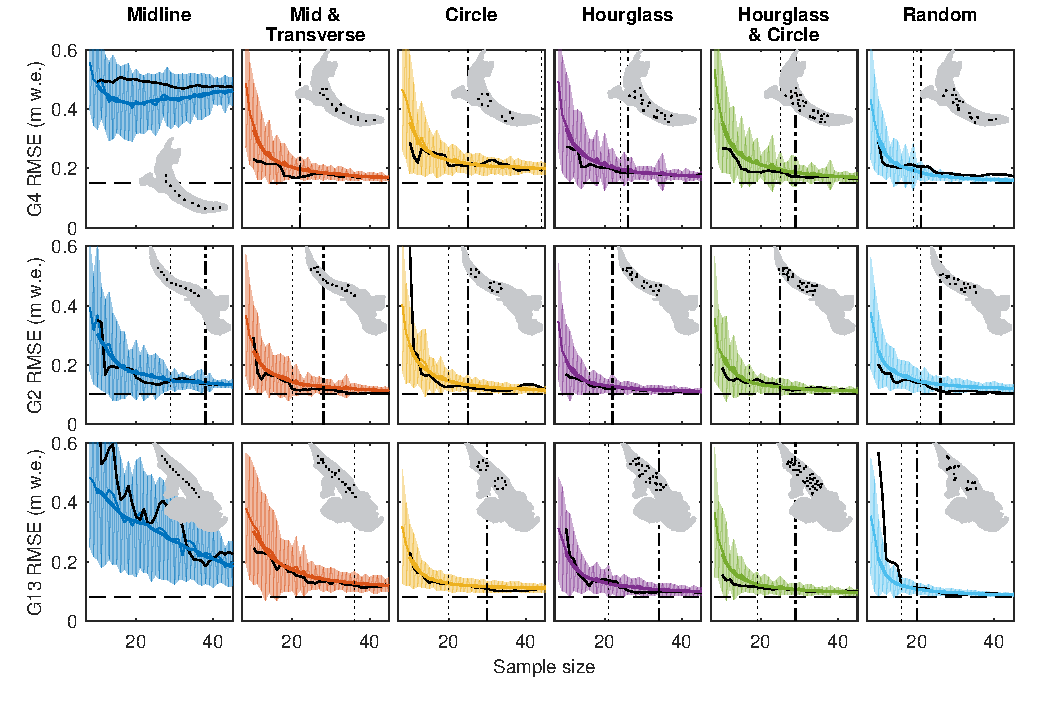
\includegraphics[width =\textwidth]{Pulwicki_Fig5.pdf}\\
	\caption{RMSE between all observed values of winter balance and the co-located estimates of winter balance using randomly selected subsets of the real data, for various sampling patterns (columns) and sample sizes (x-axes) for Glacier 4 (top row), Glacier 2 (middle row) and Glacier 13 (bottom row). Insets show example sampling schemes. Bold solid coloured lines are smoothed mean values of RMSE (fine solid coloured lines) from 100 linear regressions with randomly selected data. Shading indicates the standard deviation arising from different subsets of the randomly selected data. Solid black lines are smoothed values of RMSE from linear regressions with regularly spaced data. Horizontal dashed lines indicate the target RMSE when all available data are used to estimate winter balance.  Vertical dotted lines show sample size $n_{\rm c}$ that achieves RMSE within 5\% of the target RMSE. Vertical dot-dashed lines show sample size $n_{\rm v}$ for which the standard deviation of  RMSE (shading) comes within 25\% of target RMSE. Not all sampling patterns have $n_{\rm c}$ and $n_{\rm v}$ within the range of samples sizes shown.}
	\label{fig:RealObsWB}
\end{figure*}

%%% REAL DATA TABLE %%%%%
\begin{table*}[]
\centering
\caption{Real data tests. Ranking of survey designs from 1 to 6 (left to right) for Glaciers 4, 2 and 13 (G4, G2, G13) based on metrics (see text) $n_{\rm c}$ (top three rows) and $n_{\rm v}$ (bottom three rows). Sampling patterns are: centreline (CL), centreline and transverse (CT), circle (CR), hourglass (HG), hourglass and inscribed circle (HC) and random (RN). Colours follow figures. Values in parentheses are $n_{\rm c}$ or $n_{\rm v}$. Travel distances for each sampling pattern are given in Table \ref{tab:SynthPatternRanks}.}
\label{tab:RealPatternRanks}
\begin{tabular}{clclclclclclcl}
\hline
          && \textbf{1} && \textbf{2} && \textbf{3} && \textbf{4} && \textbf{5} && \textbf{6} \\
 \hline
                & \textbf{G4}   & \textcolor{RN}{RN}         & (19) & \textcolor{CT}{CT}         & (22)         &  \textcolor{HG}{HG}        &  (24)        & \textcolor{HC}{HC}         & (25)           &  \textcolor{CR}{CR}        & (44) & \textcolor{CL}{CL} & (--) \\
$n_{\rm c}$         & \textbf{G2}   & \textcolor{HG}{HG}         & (16)         &  \textcolor{HC}{HC}        &  (17)          & \textcolor{CT}{CT}, \textcolor{CR}{CR}        & (20)         &          &          & \textcolor{RN}{RN}         & (21) & \textcolor{CL}{CL} & (29) \\
                & \textbf{G13} & \textcolor{RN}{RN}         & (16)         & \textcolor{HC}{HC} & (19)         & \textcolor{CR}{CR}                 & (20)         &           \textcolor{HG}{HG}        &   (21)        & \textcolor{CT}{CT}         & (36) & \textcolor{CL}{CL} & (--) \\
\hline
                & \textbf{G4}   & \textcolor{RN}{RN}         & (21)         &   \textcolor{CT}{CT}        &  (22)         & \textcolor{CR}{CR}         & (25)         & \textcolor{HG}{HG}                 & (26)         & \textcolor{HC}{HC} & (29) & \textcolor{CL}{CL} & (47) \\
$n_{\rm v}$         & \textbf{G2}   & \textcolor{HG}{HG}         & (22)         & \textcolor{HC}{HC}, \textcolor{CR}{CR}         & (25)         &            &         &  \textcolor{RN}{RN}                & (26)        &  \textcolor{CT}{CT}         & (28) & \textcolor{CL}{CL} & (38) \\
                & \textbf{G13} & \textcolor{RN}{RN}         & (20)         & \textcolor{HC}{HC}         & (29)         & \textcolor{CR}{CR}                 & (30)         &  \textcolor{HG}{HG}        & (34)         & \textcolor{CT}{CT}         & (47) & \textcolor{CL}{CL} & (--) \\
\hline                
\end{tabular}
\end{table*}

\textcolor{red}{[WE SAY NOTHING OF THE REGULARLY SPACED DATA VS RANDOMLY CHOSEN HERE, BECAUSE IT'S NEW CONTENT.]}.
The RMSE between estimated and observed winter balance decreases rapidly with increasing sample size for most sampling patterns on any of the glaciers (Figure \ref{fig:RealObsWB}), with inflection points around $n=10$ in most cases. 
The performance of the sampling patterns as assessed by comparison with real data (Table \ref{tab:RealPatternRanks}) shows hourglass (HG) to rank highest for Glacier 2, and random (RN) to rank highest for Glaciers 4 and 13, for both $n_{\rm c}$ and $n_{\rm v}$. Hourglass \& circle (HC), circle (CR) and centreline \& transverse (CT) rank anywhere from 2--5, while centreline (CL) is again last in every case. 
None of the sampling patterns result in RMSE falling to that of the full dataset with $n < 45$, but random comes close for Glaciers 4 and 13, while hourglass comes closest for Glacier 2. A sample size of $n \leq 30$ is sufficient to reach the 5\% and 25\% targets for all sampling patterns excluding the centreline. 
Though the rankings in Table \ref{tab:RealPatternRanks} differ from those using synthetic data (Table \ref{tab:SynthPatternRanks}), the overall picture of performance is not dissimilar in that centreline (CL) is the only pattern that can be easily ruled out for all glaciers based on either $n_{\rm c}$ or $n_{\rm v}$.  
Note that  we have defined $n_{\rm c}$ and $n_{\rm v}$ as metrics of precision in this comparison with real data. Accuracy, in this case, is limited by the ability of the linear regression to predict observed winter balance \citep[see][]{Pulwicki2017}, with or without the use of all available data. 
    

%%%%%%%%%%%%%%%%%%%%%%%%%%%%%%%%%%%%%%%%%%%
%% DISCUSSION
%%%%%%%%%%%%%%%%%%%%%%%%%%%%%%%%%%%%%%%%%%%
\section{Discussion}

Considering $n_{\rm c}$, $n_{\rm v}$ and travel distance, the centreline \& transverse or hourglass pattern with a sample size of $\sim30$ would be leading candidates for the optimal survey design in our study region. Based on both synthetic and real data, both designs yield high accuracy or precision, are least sensitive to noise and involve relatively short travel distance. A sample size greater than 30 does not significantly improve the estimation of glacier-wide winter balance. This surprisingly low number of measurement locations indicates that high-density sampling along transects is not necessarily required in winter-balance surveys, \textcolor{red}{consistent with previous findings of annual mass balance \citep[e.g.][]{Cogley1999,Fountain1999}. }Since error is greatest in areas far from sampling locations and in areas with extreme values of topographic parameters, sampling widely throughout the study basin should be prioritized when choosing a survey design.  Based on our results, centreline is a poor choice of sampling pattern regardless of the number of measurements. \cite{Walmsley2015} suggests that winter-balance estimates require at least one measurement per 50\,m elevation band, amounting to 9--12 measurement locations on our study glaciers when only the ablation area is considered (17--24 for the full glacier). This suggestion is consistent with the $n_{\rm c}$ or $n_{\rm v}$ values for circle, hourglass and centreline \& transect sampling patterns on some of the glaciers.

Some studies of survey design for summer balance or annual (summer + winter) balance find that relatively few measurements along the centreline may be sufficient for accurate balance estimates. For example, \citep{Surjanovic2016} finds that a centreline pattern performs well in some ablation regimes, and \cite{Fountain1999} find that as few as five stakes are needed to estimate the annual balances of two small glaciers in the western continental United States.\textcolor{red}{ \cite{Fountain1999} emphasize that there is little transverse variaton in annual balance and that elevation is the dominant control on annual balance.} \textcolor{red}{MUST ALSO ESTABLISH THAT THESE GLACIERS HAVE ANNUAL BALANCES THAT CORRELATE HIGHLY WITH SUMMER BAL. DOES FOUNTAIN SAY THIS? COULD CITE OTHER LIT THAT SAYS THIS IS MORE OFTEN TRUE THAN NOT].} 
We hypothesize that a greater number of measurement locations are needed to estimate winter balance because accumulation is governed by processes that vary on shorter spatial scales than those that govern ablation \citep[e.g.][]{Dadic2010,Clark2011}. \textcolor{red}{Our work shows that adding transverse measurement locations provides a significant improvement in accuracy of winter-balance estimates.}

The most effective survey designs for our study area capture the dominant winter-balance--elevation relationship, but also sample locations characterized by a range of other topographic parameters. Although the synthetic distribution of winter balance on Glaciers 2 and 13 is largely controlled by elevation, sampling locations away from the centreline are still needed to constrain the regression. When the centreline pattern is used, the topographic parameters other than elevation are not well represented and the regression becomes sensitive to noise. This under-sampling of areas characterized by a range in the other topographic parameters also explains why increasing sample size along the centreline  does not improve accuracy as quickly as in the other sampling patterns.

For Glacier 4, the standard deviation of winter balance due to noise and the number of measurement locations needed to estimate winter balance within a prescribed precision or accuracy is smaller than for Glaciers 2 and 13. This difference is likely a result of the generally weak relationship between topographic parameters and winter balance in the synthetic distribution. The synthetic distribution of winter balance is derived from a linear regression of observed winter balance on topographic parameters that explains little of the observed variance (R$^2=$0.07) \citep{Pulwicki2017}. As a result, the synthetic glacier-wide winter balance is better explained by the mean of all observed values of winter balance than any topographic parameter. Such a spatially uniform distribution of synthetic winter balance can therefore be described with few measurements and is not sensitive to measurement location. This explains the comparatively high accuracy and precision of the Glacier 4 winter-balance estimates in the tests with synthetic data (Figure \ref{fig:SyntheticObsWB}), but the low accuracy (high RMSE) obtained in the tests with real data (Figure \ref{fig:RealObsWB}). Glacier 4 thus presents a potentially misleading picture if evaluated in isolation or only with synthetic tests.   

On average, winter balance is over-estimated with small sample sizes ($<20$), especially on Glaciers 2 and 13. We hypothesize that over-estimation results from an exaggeration of the elevation effect in the regression.
At small sample sizes, the influence of elevation over-shadows the relationships between winter balance and other topographic parameters and causes sensitivity to noise. An exaggeration of the regression coefficient results in high estimates of winter balance in the accumulation area. This result is inconsistent with that of \cite{Walmsley2015}, who found that sampling only along the centreline resulted in an underestimation of winter balance.
%[REALLY FOR WB? WHAT WAS DIFFERENT ABOUT THAT STUDY?] -> I will look into it
% DID YOU LOOK AT THE COEFFICIENTS TO MAKE SURE THE ARGUMENT ABOUT ELEVATION/OTHER PARAMS AND NOISE IS CORRECT? I DIDN'T END UP HAVING THE TIME FOR THAT YESTERDAY.

The most obvious limitation of our study is the restriction of potential survey designs to accessible locations in the ablation area. This limitation was necessitated by our dataset, which vastly under-sampled the accumulation area.
Reliable measurements of snow depth in the accumulation area are time-consuming, as detection of the snow--firn interface by probing can be difficult and must often be replaced by the excavation of snow pits. 
Such limitations can be overcome with alternative methods of measuring snow depth, such as ground-penetrating radar (GPR) \citep[e.g.][]{Machguth2006, Gusmeroli2014, McGrath2015} and repeat lidar surveys \citep[e.g.][]{Sold2013}. 
\textcolor{red}{Our work is also limited because all data arose from a single accumulation season. There is significant annual variability in snow distribution (cite!), indicating that data from additional years is needed to arrive at more general conclusions.}
Another limitation imposed by our original dataset is the fixed geographical location of the sampling patterns. An interesting extension to this study would be an examination of optimal placement of the sampling patterns. \textcolor{red}{Our work could also be extended by investiating an ensemble of synthetic distributions to test the robustness of our results. }

%%%%%%%%%%%%%%%%%%%%%%%%%%%%%%%%%%
% CONCLUSION
%%%%%%%%%%%%%%%%%%%%%%%%%%%%%%%%%%
\section{Conclusion}

Using {\it in situ} snow-depth measurements from three glaciers in the St. Elias Mountains of Yukon, Canada, we investigate the problem of optimal survey design for estimating glacier-wide winter balance. We consider six spatial sampling patterns and the full range of sample sizes permitted by our methodology and dataset. Quantitative criteria allow us to rank the performance of each sampling pattern for each glacier in tests with real- and synthetic data. A persistent result in our analysis is the inferior performance of the traditional centreline profile as a sampling scheme, even in cases where elevation is found to be the dominant topographic control on winter balance. A centreline with lateral transects, or other unconventional sampling patterns such as the ``hourglass'', yield vastly better accuracy and precision, with less sensitivity to noise. Random sampling performs almost equally well by all metrics but travel distance. The mean glacier-wide winter balance estimated with any of the sampling patterns but the centreline profile converges rapidly toward the target value with a sample size $n \sim 10$, but is consistently over-estimated at low sample sizes. In the presence of noisy or randomly selected data, performance does not generally increase for $n \gtrsim 30$. Given the relatively low required sample sizes and the value of sampling off-centreline, we suggest broad spatial coverage be prioritized over high-density sampling in surveys of winter balance.  

\section{Acknowledgements}

We thank the Kluane First Nation (KFN), Parks Canada and the Yukon Territorial Government for granting us permission to work in KFN Traditional Territory and Kluane National Park and Reserve. We are grateful for financial support provided by the Natural Sciences and Engineering Research Council of Canada, Simon Fraser University (including the KEY Big Data Initiative) and the Northern Scientific Training Program. We kindly acknowledge Kluane Lake Research Station, Sian Williams, Lance Goodwin and Trans North pilot Dion Parker for facilitating field logistics. We are grateful to Alison Criscitiello and Coline Ariagno for all aspects of field assistance and Sarah Furney for assistance with data entry. Thank you to Etienne Berthier for providing us with the SPIRIT SPOT-5 DEM and for assistance in DEM correction. We are grateful to Derek Bingham and Michael Grosskopf for assistance with statistics. 
 

%----------------------------------------------------------------------------------------
%	REFERENCE LIST
%----------------------------------------------------------------------------------------
%
%\bibliography{MastersLit.bib}
%\bibliography{MastersLit}
\bibliography{/home/glaciology1/Documents/MastersDocuments/MastersLit}
%\bibliography{/Users/Alexandra/Documents/SFU/MastersDocuments/MastersLit}
\bibliographystyle{igs}

%----------------------------------------------------------------------------------------

\end{document}
